\chapter{Die alte Anwendung}
\label{cha:ccmail}
In diesem Kapitel wird die alte Anwendung \emph{CCMail} analysiert und diskutiert. Ziel ist es, einen Überblick über diese Anwendung und deren wesentlichsten Aspekte zu liefern, sowie diese Aspekte genauer zu betrachten. Die Ergebnisse dieser Analyse sollen als Grundlage für das neue Konzept dienen, das auch die Integration in die bestehenden Anwendungen berücksichtigen muss. Diese Integration soll mit geringst möglichen Aufwand erfolgen können, da Probleme bei der Integration negative Auswirkungen auf den produktiven Betrieb haben könnten. 

\section{Systemaufbau}
\label{sec:ccmail-systemaufbau}
Im folgenden wird der Systemaufbau aus der Sicht der Anwendung \emph{CCMail} und dessen Integration in das System über \emph{MailJobs} diskutiert. 
\begin{figure}[h]
\centering
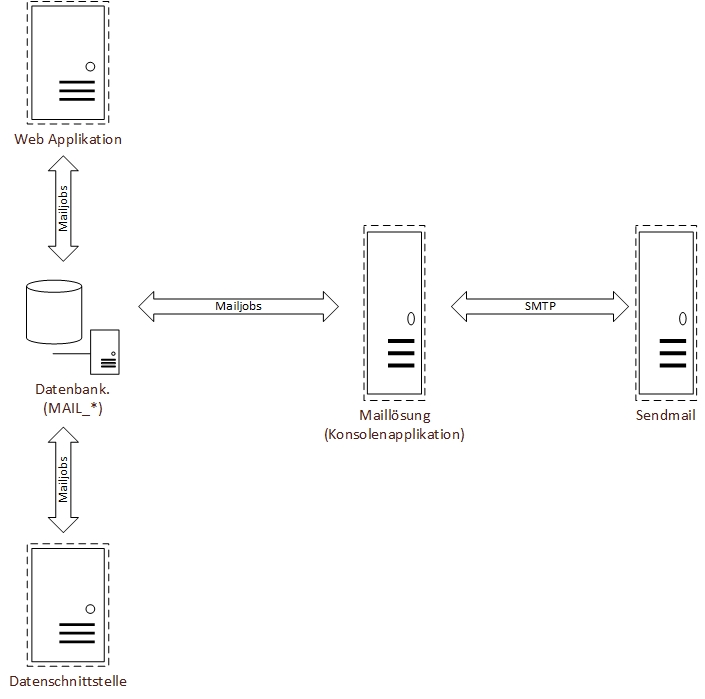
\includegraphics[scale=0.38]{Systemaufbau_alt.jpg} %{CS0031}
\caption{Systemaufbau und Integration von \emph{CCMail}}
\label{fig:ccmail-system-und-integration}
\end{figure}
\ \newpage
\parindent0pt{Abbildung} \ref{fig:ccmail-system-und-integration} zeigt das Gesamtsystem aus der Sicht der Anwendung \emph{CCMail}, wobei anzumerken ist, dass das System bis heute angewachsen ist und nunmehr aus mehreren Anwendungen als wie in Abbildung  \ref{fig:ccmail-system-und-integration} abgebildet besteht. Es lässt sich ableiten, dass das Kernstück des Systems die Datenbank ist. In der Datenbank werden die zu versendenden E-Mail-Nachrichten als sogenannte \emph{MailJobs} verwaltet. Ein \emph{MailJob} ist ein Eintrag in einer Datenbanktabelle namens \emph{MAIL\_JOBS}, die alle Informationen einer \emph{E-Mail} enthält. Es sind dabei die eigens implementierten Datenbankzugriffsschichten der einzelnen Anwendungen zu kritisieren, die zwar den Datenbankzugriff kapseln, jedoch nur für jede Anwendung an sich und nicht über Anwendungsgrenzen hinweg, was durchaus möglich wäre. Scott W.Ambler und Parmod J.Sadalge schreiben in ihrem Buch \cite[27]{refactoreDatabase} treffend:
\begin{quote}
\emph{The greater the coupeling, the harder is to refactore something. This is true of code refactoring, and it is certainly true of database refactoring}
\end{quote}
Da jede Anwendung ihre eigene Datenzugriffsschicht implementiert, muss jede Anwendung bei einer Datenbankänderung ihre Implementierung anpassen. Eine zentrale Datenbankzugriffsschicht würde nur eine Änderung an einer Stelle erfordern. Also haben wir hier eine Form der starken Koppelung die sich durch die Code-Duplikate ausprägt.
\newline
\newline
Die Anwendungen \emph{CleverWeb} und \emph{CleverInterface} erstellen über ihre eigens implementierten Datenbankzugriffsschichten \emph{MailJob-Entitäten} in der Datenbank, welche zeitgesteuert von \emph{CCMail} ausgelesen, verarbeitet und in Form von \emph{E-Mails} versendet werden. \emph{CCMail} ist als Konsolen-Anwendung implementiert und enthält alle Ressourcen, die es benötigt, um die \emph{MailJob-Entitäten} zu verarbeiten. Auch hier wirken sich die eigens implementierten Datenbankzugriffsschichten aus, da es keine einheitliche Spezifikation für das Erstellen eines \emph{MailJobs} gibt. Validierungen, ob ein zu erstellender \emph{MailJob} gültig ist, werden den einzelnen Anwendungen überlassen und sind nicht an einer zentralen Stelle umgesetzt. Daher muss sich die Implementierungen in \emph{CCMail} darauf verlassen, dass alle Anwendungen die \emph{MailJobs} korrekt anlegen, damit diese von \emph{CCMail} korrekt verarbeitet werden können.
\newline
\newline
Als Mail-Server wird \emph{Sendmail} verwendet. Es handelt sich hierbei um eine Anwendung, die für Linux Distributionen frei verfügbar ist. \emph{CCMail} versendet die \emph{E-Mails} über SMTP \emph{(Simple-Mail-Transport-Protocol)} an \emph{Sendmail}, das die \emph{E-Mails} seinerseits an die EmpfängerInnen versendet.

\newpage
\section{E-Mail-Versand}
\label{sec:ccmail-email-versand}
Der im folgenden beschriebene Prozess des E-Mail-Versands zeigt auf wie hinsichtlich des Systemaufbaus beschrieben in \ref{sec:ccmail-systemaufbau} der E-Mail-Versand vom Anlegen eines \emph{MailJobs} bis hin zum Versand der eigentlichen \emph{E-Mail} funktioniert. 
\newline
\newline
Als Kernkomponente des Systems wurde die Datenbank identifiziert, welche die \emph{MailJob-Entitäten} hält, die wiederum von \emph{CCMail} aus der Datenbank gelesen und verarbeitet werden. Dieser Ansatz ist an sich nicht als schlecht anzusehen, jedoch verbirgt sich hier eines der Hauptprobleme des E-Mail-Versandes, nämlich die Inkonsistenz der versendeten \emph{E-Mail}, durch die Zeitdifferenz zwischen dem Anlegen eines \emph{MailJobs} durch die Anwendungen und dem tatsächlichen Versand der E-Mail-Nachricht durch \emph{CCMail}.
\begin{figure}[h]
\centering
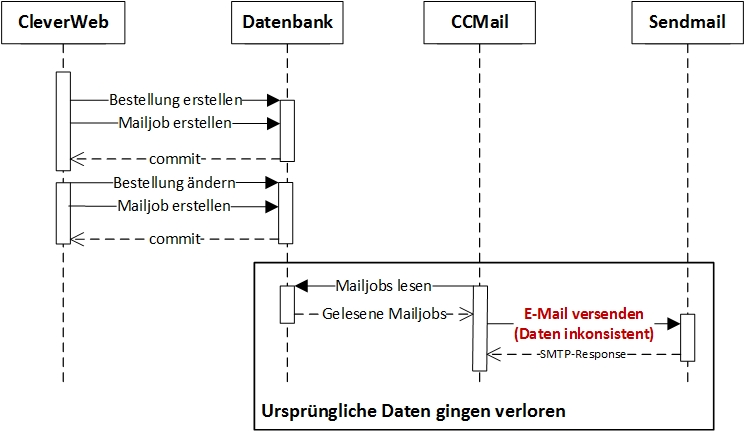
\includegraphics[scale=0.8]{prozess_sequence_emailversand.jpg}
\caption{Gesamtprozess des E-Mail-Versands}
\label{fig:sequence-diagramm-gesamtprozess}
\end{figure}
\ \newline
Wie man aus dem Sequenz-Diagramm in Abbildung \ref{fig:sequence-diagramm-gesamtprozess} ableiten kann, ist eines der Hauptprobleme am E-Mail-Versand die mögliche Inkonsistenz, was in der Art und Weise, wie die \emph{MailJob} Entitäten verarbeitet werden, begründet ist. Aufgrund der zeitgesteuerten bzw. zeitversetzten Verarbeitung kann es vorkommen, dass sich die zugrunde liegenden Daten einer \emph{E-Mail} ändern, bevor diese versendet wurde. In dem Beispiel in Abbildung \ref{fig:sequence-diagramm-gesamtprozess} wird eine Bestellung angelegt und kurz darauf geändert. Dies geschieht, bevor die \emph{E-Mail} über das Anlegen der Bestellung versendet wurde. Es wurde zwar ein neuer \emph{MailJob} angelegt, aber beide \emph{MailJob-Einträge} verweisen auf dieselbe Bestellung. Dadurch enthalten beide versendeten \emph{E-Mails} dieselben Daten und die Daten der erstellten Bestellung gingen verloren, da sie durch die gemachten Änderungen überschrieben wurden. 
\newpage
Dies ist begründet in der Art und Weise, wie die \emph{MailJob-Einträge} aufgebaut sind. Ein \emph{MailJob} hält die Daten für den Versand einer E-Mail, wobei hierbei nicht die gesamte \emph{E-Mail} oder die verwendeten Daten gespeichert werden, sondern lediglich die Parameter, die in einer SQL-Abfrage \emph{(Structured-Query-Language)} verwendet werden, um die Daten für die \emph{E-Mail} zu erhalten. Sollten sich also die Datenbank-Entitäten der involvierten Tabellen ändern, so sind die ursprünglichen Daten nicht mehr wiederherstellbar. Dadurch ist auch ein erneuter Versand einer bereits versendeten \emph{E-Mail} nicht mehr möglich bzw. es kann nicht garantiert werden, dass diese \emph{E-Mail} dieselben Daten enthält wie beim ersten Versand.
\newline
\newline
Ein weiteres Problem liegt in der zeitgesteuerten Verarbeitung der \emph{MailJobs} durch \emph{CCMail}. Lange wurde nicht geprüft, ob bereits ein \emph{CCMail-Prozess} gestartet wurde, bevor dieser erneut gestartet wird. Dies hat dazu geführt, dass es vorkam ,dass mehrere Prozesse gleichzeitig die \emph{MailJob-Entitäten} verarbeiten und daher die \emph{E-Mail} mehrmals versendet wurden. Dieses Problem ist begründet durch die Tatsache, dass in Verarbeitung stehende \emph{MailoJob-Entitäten} nicht als "\emph{In Progress}" markiert wurden und von parallel laufenden Prozessen ausgelesen und verarbeitet wurden. Nun wird zwar geprüft, ob bereits ein Prozess gestartet wurde, bevor ein neuer Prozess gestartet wird, um zu verhindern das parallel laufende Prozesse auftreten. Dies macht es aber unmöglich die Arbeit auf mehrere Prozesse aufzuteilen. Der Ansatz die \emph{E-Mails} in nur einem Prozess zu verarbeiten, hat zur Folge dass der E-Mail-Versand seriell verläuft, obwohl angemerkt sei, dass die einzelnen Nachrichten sehr wohl parallel in eigenen \emph{Threads} innerhalb des Prozesses verarbeitet und versendet werden. Man könnte die Arbeit auf mehrere Prozesse aufteilen und so die Performance verbessern und den Zeitaufwand für den Versand minimieren.

\section{Software-Design}
\label{sec:ccmail-software-design}
Nachdem der Systemaufbau diskutiert wurde befassen wir uns jetzt mit dem Software-Design von \emph{CCMail}. \emph{CCMail} wurde als Konsolen-Anwendung implementiert und stellt alle Ressourcen, die zur benötigt werden, zur Verfügung, wie:
\begin{enumerate}
	\item E-Mail-Vorlagen,
	\item Datenbankabfragen,
	\item und die implementierten E-Mail-Typen.
\end{enumerate}
\ \newline
Die Klasse \emph{CCBasicEmail} implementiert die gesamte Funktionalität für den Versand einer \emph{E-Mail} und ist die Basisklasse alle implementierten E-Mail-Typen. Die Klasse \emph{CCMailingDao} implementiert alle Datenbankabfragen über alle E-Mail-Typen hinweg. Diese beiden Klassen enthalten die gesamte Logik für die Verarbeitung eines \emph{MailJob} und des Versand einer \emph{E-Mail}.
\begin{figure}[h]
\centering
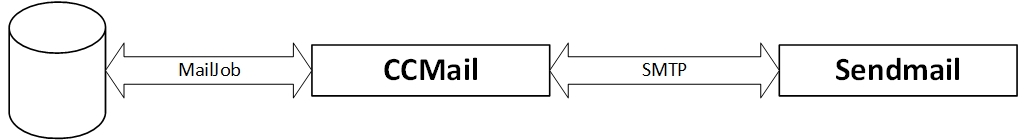
\includegraphics[scale=0.55]{teilsystem_ccmail.jpg} 
\caption{Teilsystem \emph{CCMail}}
\label{fig:ccmail-teilsystem}
\end{figure}
\ \newline
Der folgende Abschnitt wird die Schwächen der bestehenden Implementierung und deren Design analysieren. Die Ergebnisse dieser Analyse müssen bei der Erstellung des neuen Konzeptes mit einfließen und verhindern dass bereits gemachte Fehlentscheidungen sich wiederholen, sowie gute Ansätze weiterverfolgt werden.
\newline
\newline
Um das Design von \emph{CCMail} zu illustrieren wird im Folgenden näher auf die auf die Softwarekomponenten von \emph{CCMail} eingegangen. \emph{CCMail} besteht aus den folgenden Klassen:
\begin{enumerate}
	\item\emph{CCBasicEmail} ist die Basisklasse aller E-Mail-Typen, die als abgeleitete Klassen von \emph{CCBasicEmail} implementiert wurden. Sie enthält alle bereitgestellten Funktionalitäten.
	\item\emph{CCMailingDao} ist die Schnittstelle zur Datenbank, welche alle SQL-Abfragen über alle E-Mail-Typen hinweg enthält
	\item\emph{CCMailingFactory} ist die \emph{Factory-Method-Klasse} für das Erstellen von \emph{CCMailingDao} Objekten.
\end{enumerate}
\newpage

\subsection{Klasse \emph{CCBasicEmail}}
\label{sec:implementierung-ccbasic-mail}
Einleitend wird die Vererbungshierarchie der Klasse \emph{CCBasicEmail} diskutiert, welche die Basisklasse aller E-Mail-Typen darstellt.
\begin{figure}[h]
\centering
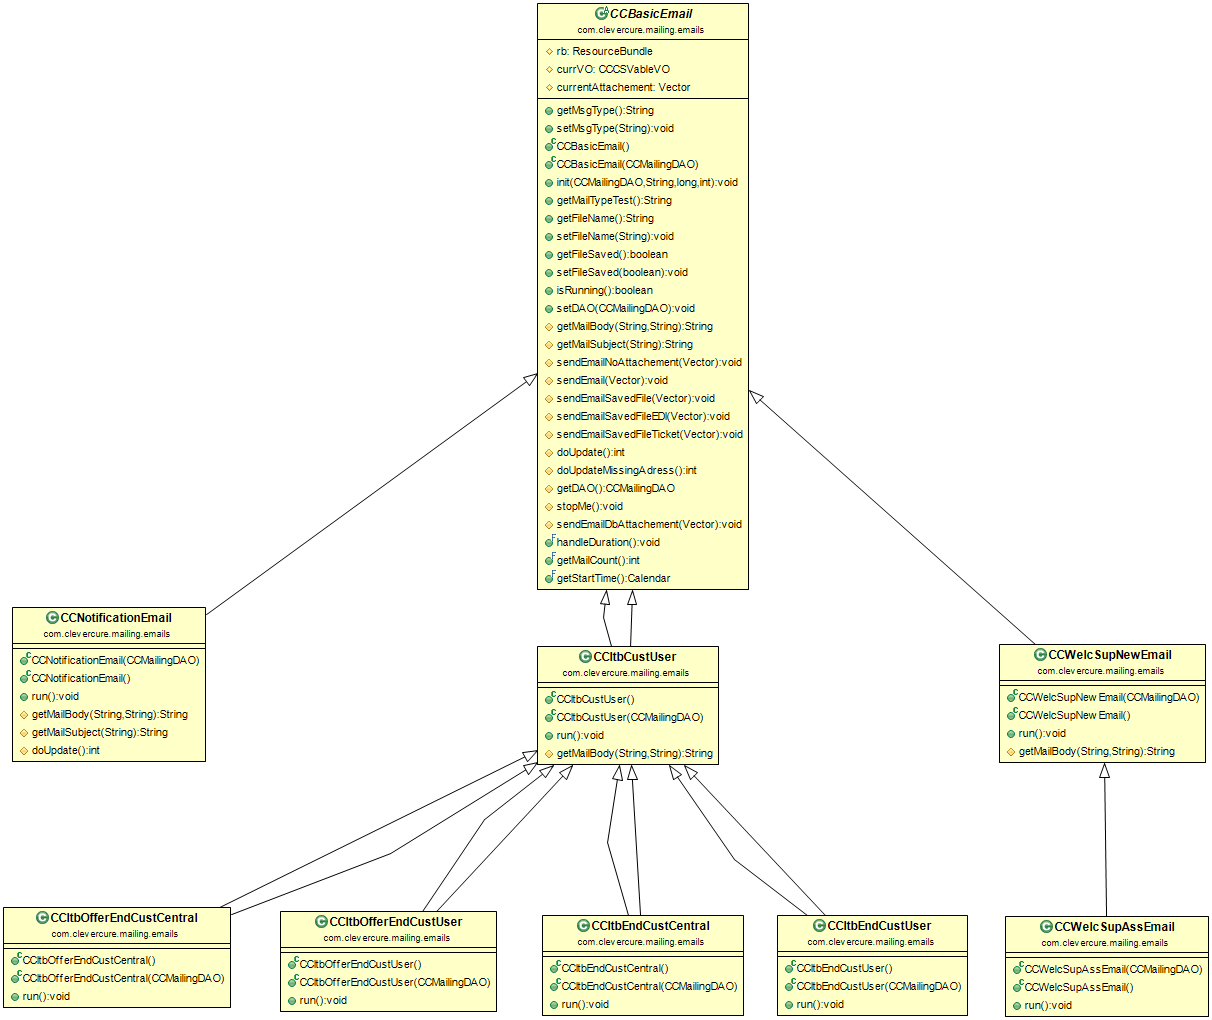
\includegraphics[scale=0.55]{class_diagram_basic_email.png} 
\caption{Auszug aus der Vererbungshierarchie von \emph{CCBasicEmail}}
\label{fig:klassen-hierarchie-ccbasicemail}
\end{figure}
\ \newline
Aus dem Klassendiagramm in Abbildung \ref{fig:klassen-hierarchie-ccbasicemail} lässt sich ableiten, dass die einzelnen E-Mail-Typen als eigene Klassen abgebildet wurden. Somit ist jeder E-Mail-Typ auch als eigene Java-Klasse abgebildet. 
\newline
\newline
Am Beispiel der Klasse \emph{CCItbCustUser} ist ersichtlich, dass neben dem Abbilden eines E-Mail-Typs als eigene Java-Klasse man ebenfalls eine eigene Subvererbungshierarchie eingeführt hat, um E-Mail-Typen, die sich in einem gemeinsamen Kontext befinden, zu gruppieren. Ob dies ein guter Ansatz ist, um kontextabhängige Ressourcen zu gruppieren, ist zu hinterfragen. Es gäbe hier andere Ansätze, wie man eine solche Gruppierung hätte realisieren können, die flexibler sind als eine Vererbungshierarchie. Eine Vererbungshierarchie ist starr und Änderungen an der Struktur können sich negativ auf die Gesamtstruktur auswirken. Ebenso produziert man so eine Vielzahl von Klassen, die gewartet werden müssen und die Struktur einer Subvererbungshierarchie lässt sich nur über ein Klassendiagramm darstellen und ist nicht aus dem Quelltext abzuleiten. Ebenso wird man bei den Vererbungshierarchien schnell an Grenzen stoßen, da hier nur gerichtete Graphen möglich sind und Mehrfachvererbung bei Klassen von Java nicht unterstützt wird. 
\newline
\newline
Mehrfachvererbung, auch wenn unterstützt, ist aber ohnedies zu vermeiden, da hier Kollisionen bei den Klassenvariablen und Methoden auftreten können. Außerdem wird durch Mehrfachvererbung die Komplexität der Klassenhierarchie nur unnötig erhöht und bringt daher keine Erleichterungen mit sich.

\subsection{Klasse CCItbCustUser}
Nachdem die Vererbungshierarchie von \emph{CCBasicEmail} diskutiert wurde, wird im Folgenden als Beispiel einer Implementierung von \emph{CCBasicEMail} die Implementierung der Klasse \emph{CCItbCustUser} angeführt. Diese Implementierung dient als Beispiel für die restlichen E-Mail-Typ-Implementierungen, die nach dem selben Prinzip mit ähnlichem Umfang implementiert wurden. Im Abschnitt ~\ref{sec:implementierung-ccbasic-mail} wurde behauptet, dass diese Ableitungen eingeführt wurden, um E-Mail-Typen zu gruppieren. Man könnte aber auch annehmen, dass diese eigene Subvererbungshierarchie eingeführt wurde, um gemeinsame Funktionalitäten für die abgeleiteten E-Mail-Typen zu kapseln. 
\newline
\newline
Folgender Quelltext illustriert, dass die Implementierungen der einzelnen E-Mail-Typen hauptsächlich aus dem Erstellen der \emph{E-Mails} besteht, da der Versand bereits in der Klasse \emph{CCBasicEmail} implementiert wurde. Die Parameter für die Vorlage werden aus dem Resultat der spezifischen SQL-Abfrage in der Methode \emph{getMailBody} extrahiert und in der Nachricht bzw. der verwendeten Vorlage verwendet. Die erstellte Nachricht wird dann als Resultat geliefert. Das unterschiedliche Erstellen der \emph{E-Mails} ist also der Grund für das Abbilden der einzelnen E-Mail-Typen als eigene Java-Klassen. Dieser Ansatz produziert viele Klassen, die in einer starren Hierarchie gebunden sind. Und dies nur um das Erstellen der eigentlichen E-Mail-Nachricht in einer eigenen Java-Klasse zu kapseln. Es sei angemerkt, dass diese Klassen auch dazu verwendet um die E-Mail-Typen zu aktivieren oder zu deaktivieren. Zu kritisieren ist hierbei, dass das Erstellen einer \emph{E-Mail} zu stark an einen E-Mail-Typ gekoppelt ist und es hier an Abstraktion fehlt. Die \emph{E-Mail} werden immer nach dem selben Schema erstellt. Es gibt lediglich folgende Unterschiede:
\begin{itemize}
	\item SQL-Abfrage, welche die Daten aus der Datenbank bezieht.
	\item Die zugrunde liegende E-Mail-Vorlage.
	\item Die Paramter für die zugrunde liegende E-Mail-Vorlage.
	\item Der eindeutige Schlüssel, der den E-Mail-Typ identifiziert.
\end{itemize}
\begin{program}
\begin{JavaCode}
public class CCItbCustUser extends CCBasicEmail {
	
	private Map cache = new HashMap();

	// empty constructor
	public CCItbCustUser() {
		super();
	} // end constructor
	
	// sets the used dao implementation
	public CCItbCustUser(CCMailingDAO dao) {
		super(dao);
	} // end constructor

	// The unique key for this email type
	@Override
	String getMailType() {
		return "ISCU";
	} // end getMailType
	
	// Thread.run method which creates and sends the email
	@Override
	public void run() {
		try {
			sendEmailNoAttachement(getDAO().getItbStartCustUserMailText());
		} catch (DAOSysException ex) {
			LOG.error("DAOSysException in CCItbCustUser.run: ", ex);
		} finally {
			stopMe();
		} // end try-catch-block
	} // end run
	
	// Method which creates the email body
	@Override
	protected String getMailBody(String bodyKey, String bodySQLKey)
		throws DAOSysException {
		int lanId   = ((CCItbVO)currVO).getLanguageId();
		int itbhId  = ((CCItbVO)currVO).getItbhID();
		String body = "";
		String key  = itbhId + "_" + lanId;
		if (cache.containsKey(key)) {
			body = (String)cache.get(key);
			LOG.debug("48: Got from cache key: " + key 
					  + " body: " + body);
		} else {
			Object[] allParams = getDAO().getItbCustData((CCItbVO)currVO, 19);
			MessageFormat form = new MessageFormat(rb.getString(bodyKey)
			                                         .trim());
	 		body               = form.format(params);
	 		cache.put(key, body);
	 		LOG.debug("48: DB access for the key: " + key
	 				+ " got body: " + body);
		} // end if-else
		return body;
	} // end getMailBody
}
\end{JavaCode}
\caption{Implementierung \emph{CCItbCustUser}}
\label{fig:code-ccitbcustuser}
\label{CCItbCustUser.java}
\end{program}
\newpage
Die folgenden drei Methoden werden von den E-Mail-Typ-Klassen implementiert:
\begin{enumerate}
	\item\emph{getMailType}: zum Bereitstellen eines eindeutigen Schlüssels, der diesen E-Mail Typ identifiziert.
	\item\emph{getMailBody}: zum Erstellen der \emph{E-Mail} aus einer Vorlage, welche mit Parametern befüllt wird
	\item\emph{run}: Jeder E-Mail-Typ wird in einem eigenen Thread abgearbeitet. Dabei wird entschiedenen welche Art von E-Mail-Versand genutzt wird. \emph{CCBasiEmail} stellt mehrere Implementierungen zur Verfügung z.B.:
	\begin{itemize}
		\item ohne Anhänge, 
		\item mit Anhängen, welche über das lokale Filesystem zur Verfügung gestellt werden, und
		\item mit Anhängen, welche über externe Systeme zur Verfügung gestellt werden.
	\end{itemize}
\end{enumerate}
\ \newline
Der Quelltext aus Abbildung \ref{fig:code-ccitbcustuser} illustriert, dass die E-Mail-Typen keine nennenswerte Logik haben, sondern lediglich für das Erstellen der E-Mail-Nachricht verantwortlich sind. 

\subsection{Klasse CCMailingDao}
Im Gegensatz zur Strukturierung der E-Mail-Typen hat man sich bei der Datenzugriffsschicht nicht dazu entschieden, diese kontextabhängig zu gruppieren. Hier wurden alle Datenbankabfragen in einer einzigen Schnittstelle spezifiziert, ohne Rücksichtnahme auf deren Kontext.
\newline
\begin{figure}[h]
\centering
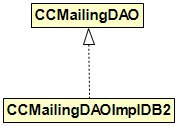
\includegraphics[scale=0.55]{class_diagram_mailing_ao.png} 
\caption{Vererbungshierarchie von \emph{CCMailingDao}}
\label{fig:klassen-hierarchie-ccmailingdao}
\end{figure}
\ \newline
Die Vererbungshierarchie aus Abbildung \ref{fig:klassen-hierarchie-ccmailingdao} ist sehr einfach, da man sich hier nicht für eine Aufteilung der Datenbankzugriffsschicht für die einzelnen E-Mail-Typen entschieden hat. Dabei ist zu bemängeln, dass sich alle Datenbankabfragen über alle E-Mail-Typen hinweg befinden und man es versäumt hat hier Schnittstellen einzuführen, welche die kontextabhängigen Datenbankabfragen spezifizieren,  also eine Schnittstelle für jeden E-Mail-Typ. Mit einer Aufteilung auf mehrere Schnittstellen hätte man die Wartung der Datenbankabfragen vereinfacht. Mit dem Ansatz der Aufteilung auf mehrere Schnittstellen, wäre man einerseits gezwungen Präfixe für die Methodennamen einzuführen, da Namenskollisionen sehr wahrscheinlich sind, und andererseits muss man darauf Acht geben, bestehende Implementierungen bei einem Restrukturieren einer oder mehrerer kontextabhängigen Implementierungen nicht zu verändern. 
\newline
\newline
Alle Implementierungen nutzen dieselben Ressourcen und müssen daher auf den kleinsten gemeinsamen Nenner zusammengeführt werden, oder man führt wiederum eigene Ressourcen ein, die sich durch ihren Namen unterscheiden. 
\newline
\newline
Eigene Schnittstellen und Implementierungen je E-Mail-Typ hätten es ermöglicht, für jeden dieser E-Mail-Typen Ressourcen zur Verfügung zu stellen, die nur dieser E-Mail-Typ verwendet. Mann hätte Flexibilität erhalten und hätte sich trotzdem auf eine gemeinsame Basis einigen können. 
\newline
\newline
Der Ansatz, die Implementierungen von \emph{CCMailingDAO} für verschiedene Datenbanken zu zur Verfügung zu stellen, ist an sich gut, jedoch hätte man sich mit der Nutzung von ORM \emph{(Object Relational Mapping)} das Leben erleichtern können, da ein \emph{ORM-Provider}, wie z.B.: \emph{Hibernate}, bereits die zugrunde liegende Datenbank abstrahiert. Datenbank-spezifische SQL-Anweisungen und Funktionalitäten werden zwar von den \emph{ORM-Providern} nicht zur Verfügung gestellt, jedoch sind solche spezifischen Teile in \emph{CCMail} nicht zu finden. Die Entscheidung, sich hier auf native SQL-Abfragen zu stützen, bringt das Problem mit sich, dass die zugrunde liegende Datenbank nicht von der Anwendung abstrahiert ist und man sich so an eine spezielle Datenbankimplementierung bindet.

\subsection{Klasse \emph{CCMailingDaoFactory}}
Zu kritisieren ist auch die Art und Weise wie ein Objekt von \emph{CCMailingDao} erzeugt wird. Man nutzt hier das Softwaremuster \emph{Factory-Method}, jedoch wird statisch die zu verwendende Implementierung in \emph{CCMailingDaoFactory} definiert, was das Austauschen der Implementierung zur Laufzeit unmöglich macht. Man hätte dies konfigurierbar machen sollen, z.B über eine Konfigurationsdatei, die den zu verwendenden Implementierungsnamen zur Verfügung stellt.
\begin{figure}[h]
\centering
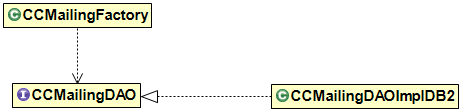
\includegraphics[scale=0.5]{class_diagram_mailing_dao_factory.png} 
\caption{\emph{CCMailingDaoFactory} für \emph{CCMailingDao}}
\label{fig:klassen-hierarchie-ccmailingfactory}
\end{figure}
\ \newline 
Im Buch \emph{Refactoring to patterns} \cite[72]{refactoreToPatterns} wird als Nachteil einer \emph{Factory-Method} die erhöhte Komplexität des Designs genannt, wenn eine direkte Instanziierung auch genügen würde. Nachdem die Instanziierung in der Basisklasse \emph{CCBasicEmail} erfolgt und die Ableitungen die Objekte über eine Get-Methode oder die geschützte Datenkomponente erreichen können, hätte man auf diese \emph{Factory} verzichten können, da die Abstraktion bereits über die Basisklasse \emph{CCBasiEmail} erreicht wurde. Somit ist der Formalparameter der Konstruktoren vom Typ \emph{CCMailingDAO} sinnlos und der Grund warum man dies eingeführt hat, ist nicht ersichtlich. Man hätte die Verwaltung der \emph{CCMailingDAO} Objekte in der abstrakten Basisklasse \emph{CCBaisEmail} halten sollen, ohne die abgeleiteten Klassen damit zu verschmutzen. 
\newline 
\newline
Zusätzlich befinden sich die Quelltexte der Schnittstellen zusammen mit ihrer Implementierungen in einem einzigen Projekt. Dies ist auch als ein halbherziger Versuch zu werten, die Implementierung von \emph{CCMailingDao} austauschbar zu machen. Man hätte hier die Quelltexte der Schnittstellen und der Implementierungen auf eigene Projekte aufteilen sollen. Somit hätte man die Abhängigkeit zu den konkreten Implementierungen der Schnittstellen vermieden und hätte sich nicht der Gefahr ausgesetzt, dass ein Entwickler sich direkt auf eine Implementierung beziehen könnte und daher immer gezwungen wäre, mit den Schnittstellen zu arbeiten.

\section{Datenbank}
\label{sec:ccmail-datanbank}
Abschließend wird hier der Aufbau des Datenbankschemata betrachtet, welches die Kernkomponente des Systems aus der Sicht von \emph{CCMail} darstellt. Es wurde bei diesem Schemata offensichtlich auf Fremdschlüssel verzichtet, was grundsätzlich nur in Spezialfällen anzuraten ist. In dem Buch \emph{Refactoring Database} \cite[213]{refactoreDatabase} wird als Argument für nicht verwendete Fremdschlüssel die Performance genannt, wobei in diesem Fall diese Begründung nicht standhält. Die beiden Anwendungen \emph{CleverWeb} und \emph{CleverInterface} erstellen lediglich einzelne oder wenige \emph{MailJob} Einträge auf einmal und \emph{CCMail} ist die einzige Anwendung, die diese \emph{MailJob} Einträge einmalig ausliest und verarbeitet. Also sollte in diesem Fall die Performance ohnehin kein Problem darstellen, da hier eine Vielzahl von Teilnehmer und die dadurch resultierende Konkurrenz nicht geben ist. Das Problem von nicht verwendeten Fremdschlüsseln wird in \emph{Refactoring Databases} \cite[213]{refactoreDatabase} wie folgt beschrieben.
\begin{quote}
\emph{The fundemental tradeoff is performance versus quality: Foreign key constraints ensure the validity of the data at the database level at the cost of the constraint being enforced each time the source data is updated. When you apply Drop Foreign Key, your applications will be at risk of introducing invalid data if they do not validate the data before writing to the database.}
\end{quote}
Hier müssen also die Anwendungen selbst die Konsistenz der Daten gewährleisten ansonsten könnten inkonsistente Datenbestände in der Datenbank entstehen, die nachträglich schwer zu identifizieren und zu bereinigen sind. Die Frage ist hierbei ob dieser Ansatz ein guter Ansatz ist?
\newline
\newline
Wie auch ersichtlich ist wurden die Spalten einer Tabelle mit einem Präfix versehen, der eindeutig über das gesamte Datenbankschema ist. Mann sollte annehmen dass es ausreicht dass die Spaltennamen eindeutig innerhalb des Kontextes einer Tabelle sind und nicht global über das gesamte Datenbankschema. Die Tabellen die neu eingeführt wurden und mit Fremdschlüsseln miteinander verknüpft sind werden dazu verwendet um Datei Anhänge von E-Mail-Nachrichten zu verwalten, die bereits bei der Erstellung des \emph{MailJob} erstellt wurden. Dies war ein Workaround und sollte so auch nicht mehr angewandt werden, da hier die Dateien in Base64 Kodierung verwaltet werden und die Datenbank unnötig mit Daten belasten. Sie sollten in einem File-Storage verwaltet und lediglich referenziert werden, was aber zum Zeitpunkt der Implementierung noch nicht zur Verfügung stand. 
\begin{figure}[h]
\centering
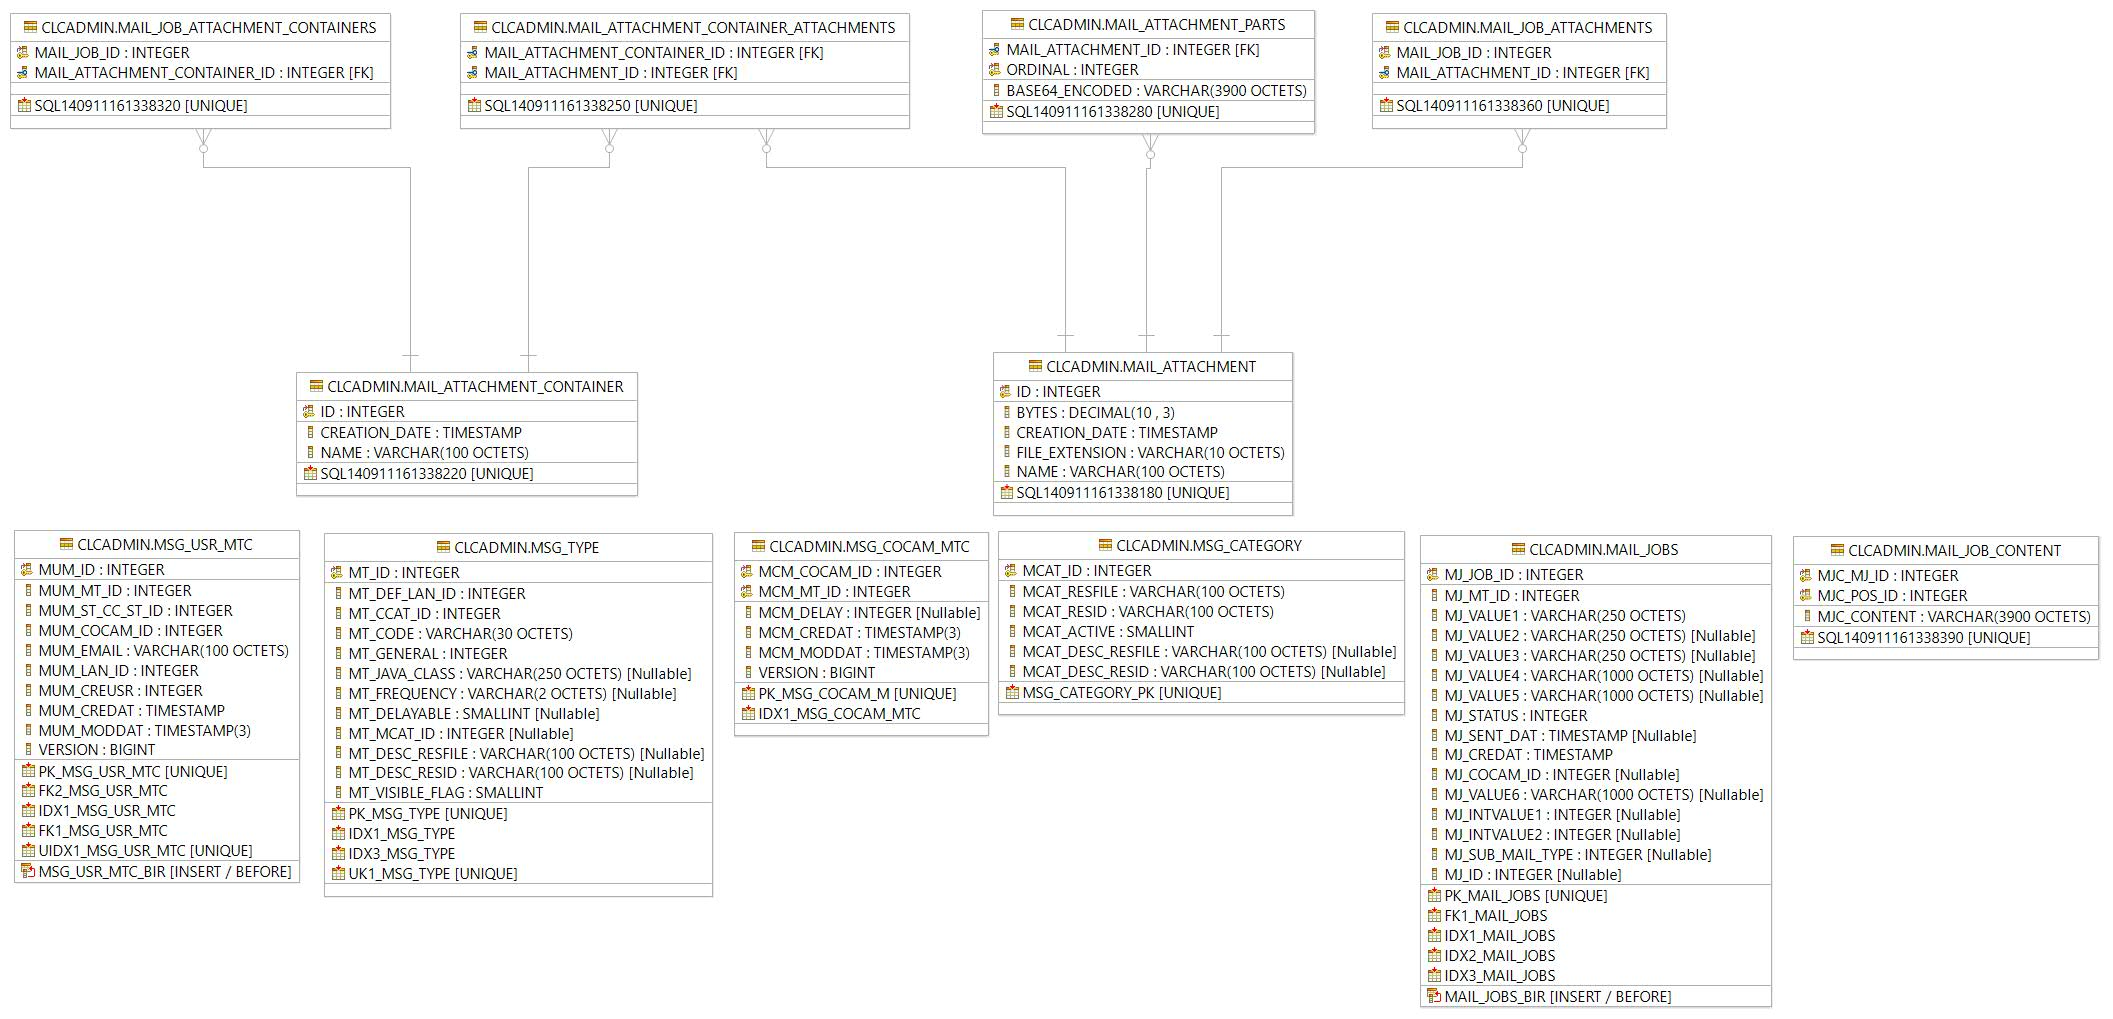
\includegraphics[angle=90,scale=0.3]{ccmail_db_schema.jpg} 
\caption{Datenbankschemata \emph{CCMail}}
\label{fig:ccmail-db-schema}
\end{figure}
